\clearpage
\twocolumn[{%
\subsection{Above-chance items}
\label{app:rq12_above_chance_items}

\noindent\begin{minipage}[t]{0.485\textwidth}
\vspace{0pt}
\paragraph{Research Question.} \emph{If every benchmark-language task keeps only the items its 1.7B runs answer above chance, how much do decision accuracy, SNR, the above-random gate and the scaling fit improve, and does it matter whether the gate is applied before or after the items are chosen?}

\paragraph{Setup.} Seed-1904 runs of every cell, 90M--1.7B, final checkpoints. Every benchmark-language task keeps only the items that its 1.7B runs answer above chance, after the above-chance gate. We compare it with the full task. The selection reads the reference by design, so the gains are an upper bound, not a held-out estimate. Decision accuracy is scored against two truths, the 1.7B ranking on the full task and on the kept items, and the gap between them is the part of the gain that comes from re-scoring the reference.
\end{minipage}\hfill
\begin{minipage}[t]{0.485\textwidth}
\vspace{0pt}
\begin{rqfinding}
\textbf{1. Keeping only the items the 1.7B runs answer above chance raises the SNR through a lower noise, not a better ranking.} The median paired SNR rises from $\times$1.27 at 90M to $\times$1.50 at 1.7B as the k-fold noise falls ($\times$0.58--0.86) and the signal stays flat ($\times$0.86--1.07), while decision accuracy barely follows, although the selection reads the reference it is scored against: the paired DA-size gain is +0.041 at 90M and +0.003 to +0.023 at 175M--1B (multi-axis pairs). (Figure~\ref{fig:app_rq12_above_chance_items}.)
\\
\\
\textbf{2. Fewer than half the items are kept.} They are 45 \% of the items of the 507 tasks the committed gate passes at 1.7B, and 44 \% over all 840 tasks with an item above chance.
\\
\\
\textbf{3. Recomputed on the kept items, the gate passes almost every task.} It passes 816 of those 840 tasks at 1.7B and 83--90 \% of the 841 at the proxies, against 37 \% (90M) to 60 \% (1.7B) for the full benchmarks: the in-sample selection all but guarantees the reference's verdict and lifts every proxy's.
\end{rqfinding}
\end{minipage}

\vspace{\baselineskip}
\noindent\begin{minipage}{\textwidth}
\centering
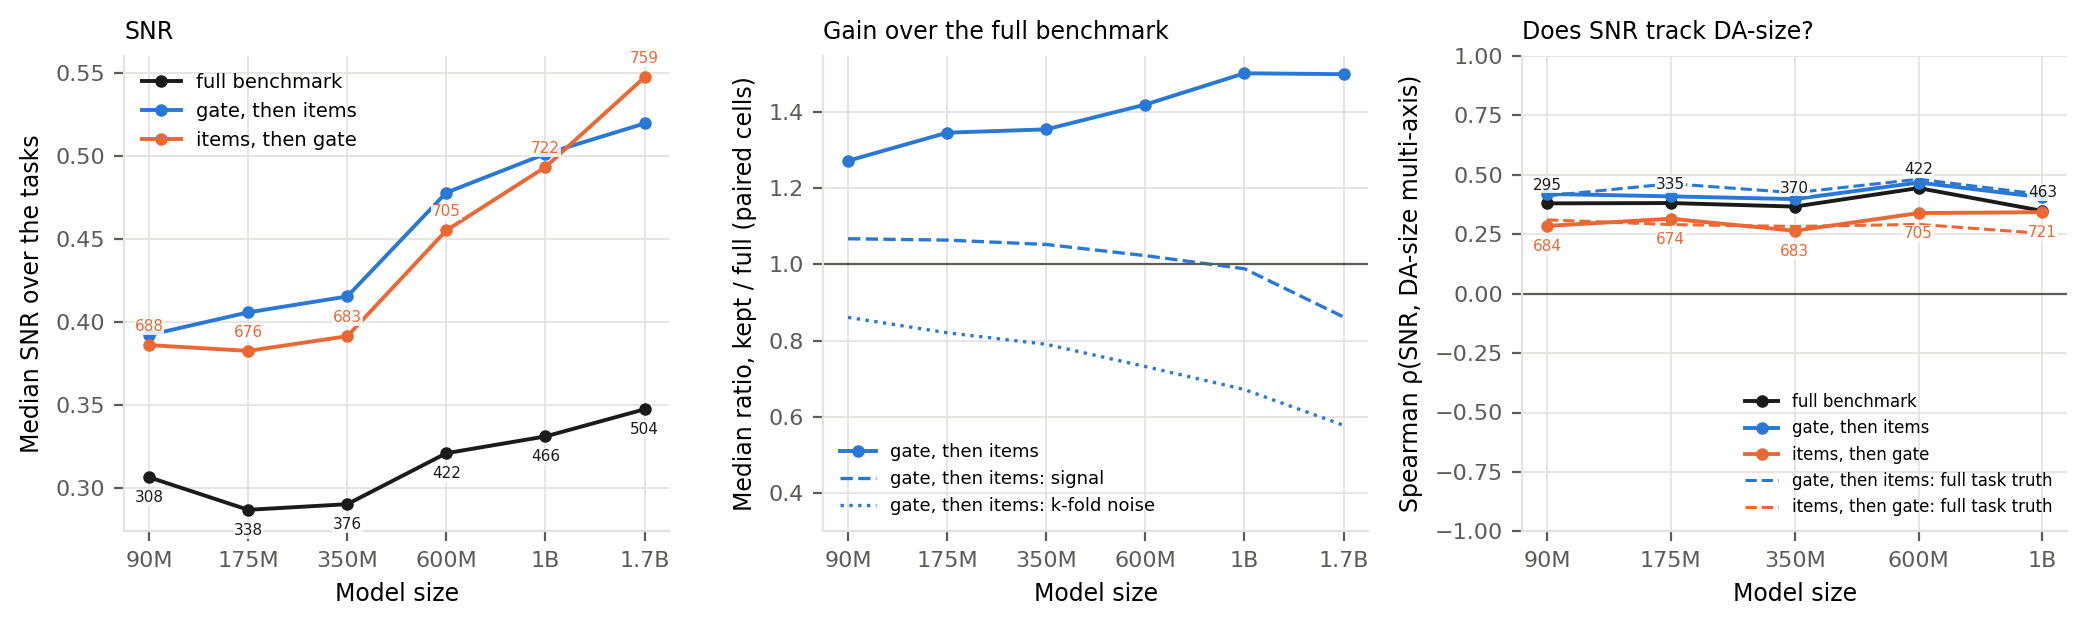
\includegraphics[width=\textwidth,height=0.36\textheight,keepaspectratio]{figures/app_rq12_above_chance_items.png}
% source: src/signal-and-noise/analysis/rq12_above_chance_items/pretraining/predictivity/above_chance_items_snr_paper.png
\captionof{figure}{\textbf{Keeping only the items the 1.7B runs answer above chance raises the SNR through a lower noise, not a better ranking.} Left: median SNR over the tasks of the full benchmark (black), of the above-chance items selected after the gate (blue) and of the gate applied after the selection (orange), per model size. The numbers give the tasks behind each point. Middle: the median ratio of the selected items to the full benchmark for the SNR, the signal and the k-fold noise. Right: Spearman $\rho$ between SNR and DA-size across tasks.}
\label{fig:app_rq12_above_chance_items}
\end{minipage}
\vspace{\baselineskip}
}]
